% CVPR 2022 Paper Template
% based on the CVPR template provided by Ming-Ming Cheng (https://github.com/MCG-NKU/CVPR_Template)
% modified and extended by Stefan Roth (stefan.roth@NOSPAMtu-darmstadt.de)
\documentclass[10pt,twocolumn,letterpaper]{article}

%%%%%%%%% PAPER TYPE  - PLEASE UPDATE FOR FINAL VERSION
%\usepackage[review]{cvpr}      % To produce the REVIEW version
% \usepackage{cvpr}              % To produce the CAMERA-READY version
\usepackage[pagenumbers]{cvpr} % To force page numbers, e.g. for an arXiv version
% Include other packages here, before hyperref.
\usepackage{graphicx}
\usepackage{amsmath}
\usepackage{amssymb}
\usepackage{booktabs}


% It is strongly recommended to use hyperref, especially for the review version.
% hyperref with option pagebackref eases the reviewers' job.
% Please disable hyperref *only* if you encounter grave issues, e.g. with the
% file validation for the camera-ready version.
%
% If you comment hyperref and then uncomment it, you should delete
% ReviewTempalte.aux before re-running LaTeX.
% (Or just hit 'q' on the first LaTeX run, let it finish, and you
%  should be clear).
\usepackage[pagebackref,breaklinks,colorlinks]{hyperref}


% Support for easy cross-referencing
\usepackage[capitalize]{cleveref}
\crefname{section}{Sec.}{Secs.}
\Crefname{section}{Section}{Sections}
\Crefname{table}{Table}{Tables}
\crefname{table}{Tab.}{Tabs.}


%%%%%%%%% PAPER ID  - PLEASE UPDATE
\def\cvprPaperID{*****} % *** Enter the CVPR Paper ID here
\def\confName{CVPR}
\def\confYear{2022}


\begin{document}

%%%%%%%%% TITLE - PLEASE UPDATE
\title{Beating the House: Deep Learning and Volatile Data}

\author{Rishabh Jain, Samarth Venkatesh\\
University of Washington\\
{\tt\small jrishabh@uw.edu, samnsid7@uw.edu}
% For a paper whose authors are all at the same institution,
% omit the following lines up until the closing ``}''.
% Additional authors and addresses can be added with ``\and'',
% just like the second author.
% To save space, use either the email address or home page, not both
% \and
% Second Author\\
% Institution2\\
% First line of institution2 address\\
% {\tt\small secondauthor@i2.org}
}
\maketitle




\maketitle

%%%%%%%%% ABSTRACT
%\begin{abstract}
    %lorem ipsum
%\end{abstract}

%%%%%%%%% BODY TEXT

%-------------------------------------------------------------------------
\section{Abstract}

\begin{abstract}
    % We look into the relation between feature selection and effective predictions in situations with data volatility. We choose our medium to be basketball, since the performance of teams is not guaranteed year after
    % year, and aim to predict match outcomes. 
    % Initial results indicate over 85\% of games' winners are accurately predicted with training on just 5 years' data on a small model using 21 features. However, this uses features of games to predict
    % game outcomes; With further experimentation, we hope to uncover a link between features and features chosen and accuracy of predictions
    % and use existing data to predict the outcome of future games
    % and ultimately beat the odds in over/under betting.

    We look into using deep learning to effectively predicting outcomes where data is highly volatile. We use the medium of basketball to determine the outcome of basketball games and predicting the winners and losers. We show and discuss some of the difficulties that arise when training volatile data and potential methods to mitigate these.
\end{abstract}

%-------------------------------------------------------------------------
\section{Introduction}
\label{sec:intro}

Predicting the outcomes of sports have been a popular activity both recreationally and professionally since the inception of professional sports leagues. Team General Managers find it important to ascertain their chances of victory or defeat in a given match to create better strategies while casual fans predict outcomes of their favorite sports team for both leisure and the prospect of making money on bets. With the advent of sports statistics tracking, it has now become possible to follow a more scientific and data-driven approach to these predictions and with the recent legalization of sports betting, these activities have exploded in popularity. \\

Of particular interest for these prediction models is deep learning. Deep learning is particularly well suited to this area due to it being able to process the large volume of statistics tracked by a sports league on its players and teams and uncover patterns that may be obscure to the human eye. Of all the popular sports with wide spread statistics present, basketball is perhaps the most well suited to this problem, owing to its vast amount of games played in a season ($2460$) as well as widely available statistics tracking everything from shot data to off court value. \\ 

Due to the nature of basketball, with occurrences like player trades and drafts, teams are subject to change every year and performance can be volatile. There is no guarantee that a team which performs well now will perform just as well within even the next year (for instance the top team in $2019$ NBA top team were the Los Angeles Lakers, who just a year back in $2018$ were the $10th$ best team). Additionally, although data regarding teams may exist starting from the $1980s$, it is hardly a good idea to use these ancient statistics when training a model for today's use due to changes in officiating and player strategy (most drastically with the wide spread adoption of $3$ point shooting post $2016$) \cite{BBR}; in other words, more data may result in worse predictions and, as a result, good feature selection is of key importance to creating an effective model for outcome prediction. As a result, this specific problem provides good insight into solving similar tasks that are constrained by volatile data and cannot be solved easily by technological improvements with respect to scaling of data. \\

We aim to explore the possibility of using deep neural networks to predict basketball game outcomes with relatively high variance in order to determine how to effectively predict game outcomes. We will demonstrate some interesting results caused by the volatility of the data - such as training less leading to better predictions - and hypothesize on some other ways to lessen the issues that arise from volatility. We believe the results will be useful in applying deep learning to other tasks such as materials machine learning or evaluating price dynamics with initial public offering. \\

% and provide an insight into creating human understandable models which provide an insight into designing smaller models before scaling up.

%-------------------------------------------------------------------------
\section{Related Work}

The paper `Predicting Margin of Victory in NFL Games' \cite{Warner} demonstrates the viability of using a machine learning based approach to outperform Las Vegas linemakers at predicting the outcome of NFL football games. Using a Gaussian process for inference, the model would recommend games to bet on. The model also makes use of non game features such as temperature of the field during play in its predictions. While the model was a good proof of concept, successfully predicting the game winner $64\%$ of the time for training data, it was only able to place successful bets under $51\%$ of the time, shy of the break even threshold. This may have been due to the scarcity of NFL game data points, since there are only $272$ total games in an entire season. Additionally, using a Gaussian Process may be an ineffective choice for modelling complex, chaotic systems like an NFL game since they struggle with high-dimensional inputs for covariance modeling and function estimation \cite{GP}. Finally, the feature selection itself may have also been inappropriate, owing to the amount of correlation in certain features and weak correlation with other features (such as the temperature of field at time of play). In $2010$, it was difficult to receive individual team statistics, which would have made it difficult to effectively predict the next victories or losses for a team due to the high predictive power of certain features. \\

Another paper, `Football Match Prediction using Deep Learning' \cite{Pettersson} uses a recurrent neural network model to predict the outcome of soccer matches. The architecture  uses a Long Short Term Memory Network that processes game data at a given time step, enabling the authors to receive a live prediction of a game winner with the progression of the match. At the start of games, with no information about the incoming match, the prediction accuracy is $34.30\%$ for the many-to-one model and $45.90\%$ for the many-to-many model, but as more information is received by the network (i.e. later in-match statistics are provided) the better the network performed on predicting the outcome. At full time the many-to-one reached $98.63\%$ test accuracy and many-to-many model had $88.68\%$. While the high accuracy of the model seems promising, the glaring issue with this approach is its poor accuracy at the start of matches, which is when most sports betting is allowed; the high accuracies for a given match outcome are achieved using data from the match being predicted itself, which makes the model less useful for predictions. This poor accuracy at the start of games, when little information about the game is provided is a result of Long Short Term Memory Networks being fundamentally unsound for non sequence classification problems (and the prediction of sports outcomes is not a sequence classification problem due to its fixed length inputs and outputs). Additionally, Long Short Term Memory Networks are computationally complex, requiring a lot of time to train. Finally, due to the correlation between certain statistics in sports as well as the sheer volume of confounders in a sports game, the parameters chosen by an recurrent neural network or Long Short Term Memory Network will almost assuredly result in an overfitted model, which results in a bad prediction. \\

A third paper, `Sports Betting: an application of neural networks
and modern portfolio theory to the English Premier
League' \cite{Jiménez} presents a novel approach combining Utility Theory with machine learning methods. In particular, it trains a deep neural network with $3$ elastic net, lasso, ridge and drop out layers and $9$ batch norm layers to estimate the odds and evaluate the odds using Kelly’s financial criteria and other methods from utility theory. The model resulted in a positive gain on investment, but also had high variance on each bet and had low diversification with each bet taken, implying that certain bets taken would result in either significant gains or significant losses, which itself implies the model is sensitive to the training data and may not generalise well. This may be as a result of the lack of training data $(380$ total matches are played in a season), but it suggests the practicality of using a neural network (specifically a deep learning) approach to sports modelling. This paper demonstrates that neural networks both converge faster and have lower bias compared to traditional supervised classification methods. Additionally, as the paper notes, another area of improvement is in feature selection, which it states to be an extremely relevant factor, resulting in faster convergence and more accuracy, less variance and lower bias for a model. \\

Finally, `Exploiting sports-betting market using machine learning' compares a convolutional neural network and neural network based approaches to sports prediction \cite{Hubáček}. The model itself consists of a convolutional layer followed by $3$ dense layers being compared to a standard (deep) feed-forward architecture with 4 dense layers. The advantage of such an approach is that it is complex enough to represent the relationships between features selected and match outcomes, finding that a deep learning based approach had faster convergence and greater accuracy than standard classification ML algorithms, but, as the paper notes, the choice of specific deep learning model (convolutional neural network vs neural network) had less impact on the accuracy of the data compared to the choice of features and volume of data provided to the models (as evident with the accuracies of both models being similar within the margin of error). 

%-------------------------------------------------------------------------
\section{Technical Challenges}

There were not too many challenges with implementing this project. The 
primary challenge was procuring the statistics. We built a
data scraper using beautifulsoup4 and playwright to scrape Basketball-Reference \cite{BBR} to procure the web pages and converted them to csv files using another script. A common challenge with scraping vast amounts of data is timeouts: since sites expect large amounts of API calls to be malicious, they often timeout the actor calling the API (in our case, our webscraper). By randomizing the time of API calls and scaling the calls to number of previous calls made, we were able to procure the data. \\

The next challenge was in pre-processing the data. Using pandas, we were
able to import the csv files, remove NA values, and extract relevant
features as desired. We designed some functions to compute running averages (discussed later) and match them with the outcome to be predicted. PyTorch enabled us to convert these into the relevant
objects to use with our model. Identifying the relevant features was difficult and relied on making educated guesses and using Dean Oliver's Basketball on Paper \cite{Oliver} to identify the most useful statistics. Once the features were identified, using built-in methods from numpy and pandas, we were able to preprocess the data satisfactorily. \\

Developing the model architecture was also a concern. From our lectures in class and our literature review, we realised that deep neural networks are likely to be the most effective model for this specific task due its ability to fit into any complex function easily and reach convergence faster than other deep learning based models such as recurrent neural networks and Long Short Term Memory Networks. The quick training time allowed us to try various things without having to bear excessive waits. \\

With regards to our model and code, we are leveraging some functions
from assignment 4 to allow for training and checking of our model.
The rest of our code is not based off of any repository and is entirely original work. \\

%-------------------------------------------------------------------------


%-------------------------------------------------------------------------


%-------------------------------------------------------------------------
\section{Methods}

% We began research by constructing a simple model using a one-layer neural net
% which we could use as a springboard for our experiments. This one-layer model
% allowed us to begin tinkering with the inputs and outputs. Since our focus is
% on finding the right combination of features to maximize accuracy, we did not
% spend much more time finding the most optimal model - a basic neural net
% was sufficient for the format of the data
% and to achieve reasonable training and validation accuracy. We compare our model to a benchmark accuracy of $75\%$ suggested by Zimmermann et al \cite{Benchmark} due to the binary nature of our prediction when finding win/loss outcomes.
% In addition, we compare the performance of our DNN to a standard regression model to identify the effectiveness of a deep learning based approach as compared to the opposite. 

% Both models took the following features (for both the player and the opponent) and predicted the the winner of a match between two teams.

We began by constructing a simple model using a one-layer neural network which served as a proof of concept for our idea. We chose the following features when training:

\begin{enumerate}
    \item True Shooting Percentage (TS\%): Shooting percentage adjusted for three-pointers and free throws. It is a measure of shooting accuracy. TS\% = Points/($2 \cdot $ Field Goal Attempts + $0.44 \cdot$ Free Throw Attempts)  \\
    \item $+/-$: Measures impact on the game by calculating the change in the score. \\
    \item $+/-$ Max Opponent: Measures highest impact on the game by calculating the change in the score. It is a measure of opponent quality. \\
    \item Offensive Rebound \% (ORB\%): Measures percentage of possessions ending in an offensive rebound. \\
    \item Defensive Rebound \% (DRB\%): Measures percentage of possessions ending in an defenseive rebound. \\
    \item Assist ratio \% (Ast\%): Measures percentage of possessions ending in a assist. \\
    \item Steal \% (Stl\%): Measures percentage of opposing team possessions ending in an steal . \\
    \item Block \% (Blk\%): Measures percentage of opposing team possessions ending in an block. \\
    \item Turnover \% (Tov\%): Measures percentage of possessions ending in an turnover. \\
    \item $3$ Points attempted per Field goal attempt ($3$Par): Number of $3$ point attempts attempted per field goal attempt. \\
    \item Free Throw Rate (Ftr): Number of free throw attempts attempted per possession of ball. \\
    \item Home field Advantage (Home Opp): Shows whether the team has home field advantage or not. \\
\end{enumerate}

$9$ more features were identical versions of items $1$ and $4-11$ but for the opponent team; there are a total of $21$ features. The model predicts the win/loss of the ``current'' team.
These features were numeric aspects of a game (or could be easily represented as such) that account for both quality and quantity of a team; in other words, they account for not only the actual success of a team in attempting things such as percentage of successful shots but also the number of shots attempted, which are both important metrics. \\

This model used the statistics of each game to predict the outcome of the game and had excellent results, as expected, since it was an ex-post-facto prediction of sorts, similiar to the LSTM network dicussed earlier \cite{Pettersson}. \\

Once this base model was built, we focused on pre-processing our data to prepare it for actual predictions. This involved computing running averages of a team's statistics up to each match to use when training and testing, and labeling the average stats up to each game with the win or loss of the next game, since that is what we wished to predict. It's not very helpful to use the stats of a game that is already finished to predict that game's outcome, which was the reason for doing this. We could leverage previous matches' data to predict to the next one. \\

We also built a regression model using ridge regression with an alpha of $1$ to generate the probability of victory and loss of a game given the previous game's statistics and achieved an accuracy of $53\%$. We hypothesize that deep learning methods, particularly with running averages, will lead to better results. \\

A difference between our project and the most research in this sphere
is the lack of randomly splitting the data. Since our goal is to use
currently available data to predict future outcomes, we structured the split of our
training, validation, and testing data similarly, opting to use older
data to predict future outcomes instead of randomly choosing between
all available data at a given moment. We chose to split our data at the 2021-2022 season mark and the 2022-2023 season mark; any games before the latter were used for training, any in the latter for validation, and games in the former were used for testing. \\

Ultimately, we simply hoped to do better than the regression model and glean some insights into applying deep learning in situations with volatile data. \\

% After that, we tried different combinations of features and the effect of such
% on predicting the winner. We then repeated the described methods on predicting
% the total score of both teams in a game and gauging how effectively combinations
% of features could "beat the house" in predicting over/under bets; in other words,
% could our model effectively predict that the total score would be over or under
% the given estimate to win the bet 53\% of the time (HOW IS THIS DETERMINED).

% Although the training data uses the features of a team in a given \textit{game},
% this can hardly be used during test time; we would be using the features
% of a game to predict the outcome of the game, which is nonsensical!
% Instead, we will use the statistics of one game to predict the outcome
% of the next game. We will also compute the average statistics of a team in all games played
% up to that point in the \textit{season} (seasonal statistics to-date) and use that
% as the input data when predicting the test outcomes.
% We can then compare the efficacy of these two methods of using previous statistics.

% Ultimately, we hope to predict the total score of a match to effectively bet
% in over/under betting and making a profit. This means the predicted the actual score
% of the match and the predicted score of the match according to our model
% must \textit{both} be over or under the given value of the bet at least
% $52.4\%$ of the time. This is because at $10-11$ odds (i.e. spending $11$ dollars to win $10$ dollars), which are the median odds of an arbitrary bet, assuming we win $x$ bets and lose $1 - x$ bets, to break even we need to win $10x - 11(1 - x) = 0 \rightarrow x = 0.52387 \approx 52.4\%$ of our bets.

%-------------------------------------------------------------------------

\section{Experiments and Results}

We tested three different types of models using deep learning to see how volatile data interacted with deep learning. The three models were:

\begin{enumerate}
    \item Using the previous game's statistics to predict the next game's outcome using data from 2015-2016 season to the 2020-2021 season for training
    \item Using running averages up to each game from the 2015-2016 season onwards with training ending at the 2020-2021 season
    \item Using running averages beginning with the 2020-2021 season and only training on that season
\end{enumerate}

All three models used the 2021-2022 season as validation, the 2022-2023 season for testing, and 30 epochs for training. Ultimately, the worst performing model was the first one (figure 1), with a test accuracy of 51.85\%, failing to beat our baseline regression model. \\

\begin{figure}[htp]
    \centering
    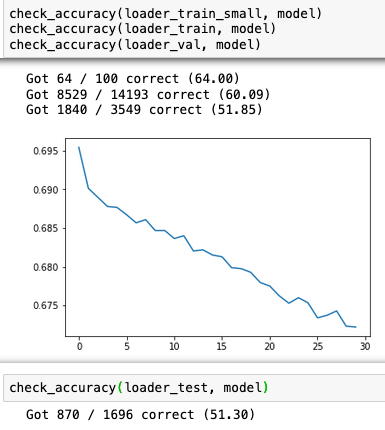
\includegraphics[width=8cm]{results_2016_train_non-avg.png}
    \caption{Loss over 30 epochs using previous game stats}
    \label{fig:fig_1}
\end{figure}

This falls in line with our hypothesis that running data is necessary for good outcomes. Using only one piece of data (such as the previous game) does not account for outliers and ``smoothing'' since there could be all kinds of differences between a team's average performance over a season and how they perform in one specific match. Using just one match also fails to account for the effect of on a team by each possible opponent, which averaging over all games accounts for. \\

Of the other two models, the one trained on only 2020-2021 matches achieved better results than the one trained on data since 2015, as indicated by figures 3 and 2 respectively. \\

\begin{figure}[htp]
    \centering
    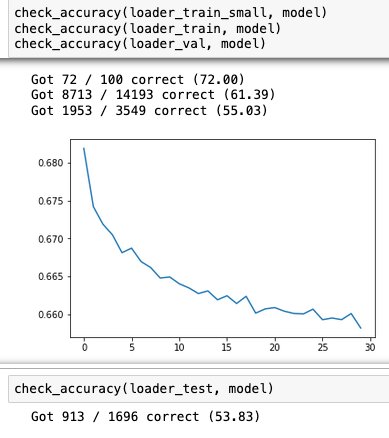
\includegraphics[width=8cm]{results_2016_train.png}
    \caption{Loss over 30 epochs using running stats since 2015}
    \label{fig:fig_2}
\end{figure}

\begin{figure}[htp]
    \centering
    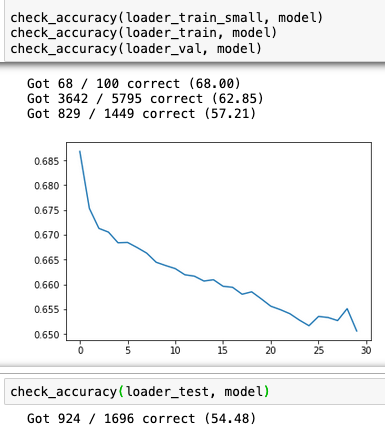
\includegraphics[width=8cm]{results_2020_train.png}
    \caption{Loss over 30 epochs using running stats since 2020}
    \label{fig:fig_3}
\end{figure}

This is somewhat surprising, since using less seasons to train means that the model is trained on less data, running against common machine learning wisdom. However, the volatility of the data in combination with the fact that basketball teams can change quite a bit in a few years may be behind this. A team's performance in the previous season is more relevant to how they will perform now compared to their performance several seasons ago. It's possible that using a decaying running mean, similar to gradient descent algorithms, could lead to even better results as more recent data will be weighted better without dropping old data (as we did), allowing the model to learn with more data. \\

Lastly, we noticed that batch normalization led to marked improvements in the results. The previously mentioned models all used batch normalization; running model 3 without batch normalization results in figure 4. \\

\begin{figure}[htp]
    \centering
    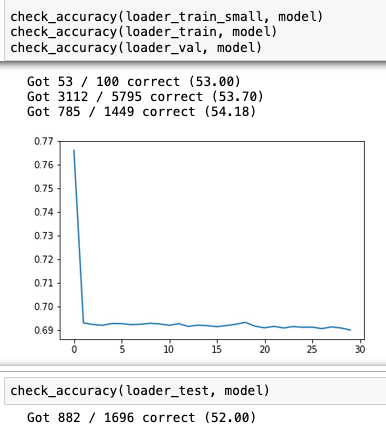
\includegraphics[width=8cm]{results_2020_train_no-bn.png}
    \caption{Loss over 30 epochs using running stats since 2020, no batch normalization}
    \label{fig:fig_4}
\end{figure}

The lack of batch normalization leads to a plateau in the decrease of the loss and the model doesn't fit even the training data very well. We think that the effectiveness of batch normalization here is due to the network becoming more robust to initialized weights as well as its regularization properties, which prevents it from making predictions based on the noise inherent to the data. We discuss the impact of this in greater depth in the next section. \\

% So far, we have only created one model using 21 features from both teams total to predict
% the team which wins. This model has 2 hidden layers of sizes 128 and 32 and an output
% layer of size 2 (win vs. loss). The validation data with current game statistics
% has just over 90\% accuracy.

% \begin{figure}[htp]
%     \centering
%     \includegraphics[width=8cm]{loss_1.png}
%     \caption{Loss over 10 epochs using current game stats}
%     \label{fig:loss_1}
% \end{figure}

% Initial results with using previous game statistics to predict next game
% statistics result in a roughly 50\% accuracy, which makes sense,
% as game statistics are highly correlated with the game outcome as opposed
% to game statistics to the next game's outcome.

% \begin{figure}[htp]
%     \centering
%     \includegraphics[width=8cm]{loss_2.png}
%     \caption{Loss over 10 epochs using previous game stats}
%     \label{fig:loss_1}
% \end{figure}

% We have additionally created a baseline model using Ridge Regression that achieves an accuracy of $53\%$ in predicting whether the next game will be a victory or a loss based on previous game(s) data.


%-------------------------------------------------------------------------

\section{Discussion}

Our results indicate some promise as they appear to correctly predict the outcome of a game with over $54\%$ accuracy without excessive hyperparameter tuning. Potential improvements in the tuning along with other modes of possible improvement could lead to even better results. We discuss some of these potential modes below. \\

One potential improvement is training on only wins. Since this cuts out half the training data, we expect training to be faster. The nature of the data is such that points labeled as ``loss'' are the same as those labeled ``win'' but with the numbers in team/opponent features swapped. If the model successfully determines how to predict wins, then as a side effect it has determined losses as well. The cost effectiveness can be achieved only because our labels are binary and the features are mirrored; if we were to use a different set of features then cutting out half the data might not be feasible. \\

% We first expect that training the model on only wins would be at least equally effective as training on both wins and losses with a faster convergence rate. This is because our data for team statistics is essentially mirrored on the other side and a given team's win is its opponent's loss. As a result, it is likely that by mirroring the data and training on only wins, the model would be able to determine what features contribute to a win, and as a side effect, it will also determine which features contribute to a loss. This is potentially interesting for binary classification problems since it may be more cost effective to train on only approximately half the training set while still achieving similar results. \\

We hypothesize that using running averages that reset at each season (rather than running averages from the very beginning of the training set) could lead to some improvement. This is because of out-of-court changes that impact game outcomes between seasons - such as player improvements due to better training and health - to more significant changes such as player trades. Weighing more recent data more heavily rather than using an unweighted average when computing the running statistics could also improve our model. As demonstrated in our experiments section, dropping earlier seasons resulted in higher test and validation accuracy and lower loss, suggesting that more recent data has a stronger correlation with recent outcomes. \\

We also note that, while our results are promising, they still aren't highly accurate, only a little better than random chance. We posit that this is as a result of other impact factors not captured in data such as player coaching and screen setting. The difficulty with capturing this data is that since it is largely intangible (the box score doesn't include these features), it is difficult to create an all encompassing model. \\

In addition to outputting game outcomes, future research may also benefit from outputting the confidence score associated with an arbitrary prediction. We note that our model only outputs the binary outcomes of a game (i.e. win or loss), but it does not return the confidence with which it made these predictions. Confidence is significant within the context of sports betting, because it enables a bettor to accurately determine the percentage of capital they should place for a given bet to maximize their long term returns. As suggested by DeVries et al in `Learning Confidence for Out-of-Distribution Detection in Neural Networks' \cite{Confidence}, one approach involves training neural network classifiers to output confidence estimates for each input, which are then used to differentiate between in and out-of-distribution datasets. \\ 

Our results show that while deep learning may be an effective tool in scenarios with volatile data, such as with stock market analysis or materials machine learning, it needs to be supplemented with non machine learning based techniques to improve its accuracy. As mentioned before, this is due to the data not necessarily capturing all the features that are relevant to a given task and because the high volatility inherent to the data results in high amount of error being associated with the model's predicted outcomes. As suggested by Jiménez et al\cite{Jiménez}, using traditional statistical methods from game theory such as Kelly criterion or data generation techniques like data imputing may mitigate issues that arise due to volatility. \\

%-------------------------------------------------------------------------


%-------------------------------------------------------------------------



%-------------------------------------------------------------------------


%------------------------------------------------------------------------

%%%%%%%%% REFERENCES
{\small
\bibliographystyle{ieee_fullname}
\bibliography{egbib}
}

\end{document}
